\documentclass[tikz,border=2pt]{standalone}
\usetikzlibrary{positioning}

% --- 重新定义颜色 (中等饱和度,清爽且可见) ---
% 选取了 PPT 风格中等强度的颜色,适合做清晰的边框
\definecolor{midOrange}{HTML}{F57C00} % 最左/最右:中橙色
\definecolor{midBlue}{HTML}{1976D2}   % 第二/第四:中蓝色
\definecolor{midTeal}{HTML}{00897B}   % 中间:中青色

\begin{document}
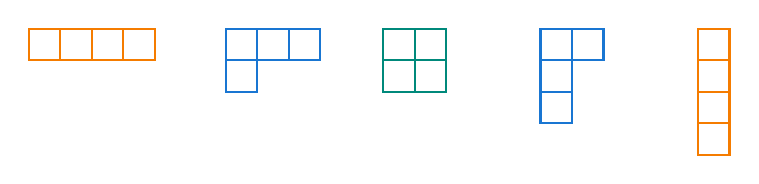
\begin{tikzpicture}[
    % 定义统一的线条样式:使用标准的 'thick' (约0.8pt),比之前的1.5pt细很多
    border_style/.style={thick}
]

    % --- 绘制宏 (保持不变) ---
    % 参数:\yd{名称}{位置}{行数据列表}{边框颜色}
    \newcommand{\yd}[4]{
        \node[inner sep=0] (#1) at (#2) {};
        \begin{scope}[shift={(#1.north west)}]
            \foreach \row [count=\r] in {#3} {
                \foreach \col in {1,...,\row} {
                    % [color=#4]: 应用边框颜色
                    % [border_style]: 应用变细后的线条样式
                    \draw[color=#4, border_style] (0.4*\col-0.4, -0.4*\r+0.4) rectangle ++(0.4, -0.4);
                }
            }
        \end{scope}
    }

    % 1. Partition [4] -> 最左边 (中橙色)
    \yd{p4}{0,0}{4}{midOrange}

    % 2. Partition [3,1] -> 第二个 (中蓝色)
    \yd{p31}{2.5,0}{3,1}{midBlue}

    % 3. Partition [2,2] -> 中间 (中青色)
    \yd{p22}{4.5,0}{2,2}{midTeal}

    % 4. Partition [2,1,1] -> 第四个 (中蓝色)
    \yd{p211}{6.5,0}{2,1,1}{midBlue}

    % 5. Partition [1,1,1,1] -> 最右边 (中橙色)
    \yd{p1111}{8.5,0}{1,1,1,1}{midOrange}

\end{tikzpicture}
\end{document}